%%% In this section, you will describe all of the various artifacts that you will generate and maintain during the project life cycle. Describe the purpose of each item below, how the content will be generated, where it will be stored, how often it will be updated, etc. Replace the default text for each section with your own description. Reword this paragraph as appropriate.

\subsection{Major Documentation Deliverables}

\subsubsection{Project Charter}

After submitting the initial project charter on 10/5/20, changes will be made in the cases where it is necessary, for example if new constrains are identified, budgetary changes take place, any developments that might take place to the system overview during the following sprints. The document will be reviewed, updated and maintained at the end of every sprint.Each member of the team will be responsible for the maintenance of the document.The final version of the project charter will be delivered in May of 2021.

\subsubsection{System Requirements Specification}

The initial system requirements specification document will be delivered in the week of 10/12/20. This document will be maintained as we work our way through the sprints and develop a better idea as to which of our requirements are realistic and can be delivered upon.Also,during our meetings with our sponsors or medical professionals if a necessary feature is brought into our attention, the document will be appended accordingly.Each member of the team will be responsible for the maintenance of the document.The final version will be delivered in May of 2021

\subsubsection{Architectural Design Specification}
The document will be updated(if need be) at the end of every sprint in the case that any developments are made to the initial design specifications or a new specification has to be added to the original list.Each member of the team will be responsible for the maintenance of the document. The final version will be delivered in May of 2021.

\subsubsection{Detailed Design Specification}
The document will be updated(if need be) at the end of every sprint in the case that any developments are made to the initial design specifications or a new specification has to be added to the original list.Each member of the team will be responsible for the maintenance of the document. The final version will be delivered in May of 2021.

\subsection{Recurring Sprint Items}

\subsubsection{Product Backlog}
Each SRS will be given a unique ID and will be added in a team-maintained sheet. Each SRS will be given a priority category, based on sponsor's preference and its important towards building the final product. The estimated cost will be decided by the team members who will be working on that branch of the product.

\subsubsection{Sprint Planning}
Each sprint will be geared towards adding more functionalities based on the SRS list and the priority given to us by the sponsor. We will have in total of about 7 sprints. 
\subsubsection{Sprint Goal}
 The Team leader will decide on how the sprint will be planned. This will be based on their planning along side inputs given by our team mates. We will be presenting our progress to  the sponsor after every sprint to keep them updated and also to take valuable inputs from them.

\subsubsection{Sprint Backlog}
The Scrum master decides which product enters the sprint backlog based on the priorities. Out team will be using, Trello, an online software, to keep track of our backlogs.

\subsubsection{Task Breakdown}
The individual tasks will be decided on team members strength by the Team leader. The time spent on a particular task will be decided based on the input received from the team member who has be assigned that particular task.

\subsubsection{Sprint Burn Down Charts}
The scrum master will be responsible to generate the Burn Down charts. After every sprint, we will report the time spent on each tasks.

\begin{figure}[h!]
    \centering
    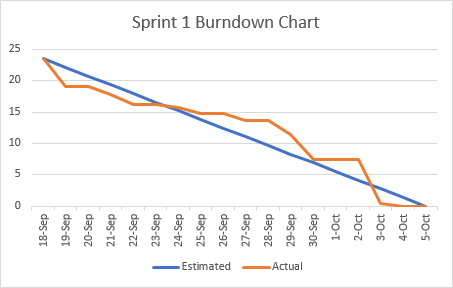
\includegraphics[width=0.75\textwidth]{images/burndown.png}
    \caption{Sprint 1 burn down chart}
\end{figure}

\subsubsection{Sprint Retrospective}
The Scrum master will be responsible for the sprint retrospective. We will be meeting every week as a part of out touchbase meeting to discuss what we did for the previous week and any difficulties that we faced during that. We will be documenting our progress as a group and also individual milestones that everyone can set on their own during the meeting. Everything we do on a sprint will be due when the sprint ends.

\subsubsection{Individual Status Reports}
Each individual will be required to submit all the SRS they worked on and their progress on it. The key items that will be discussed in this report will be any difficulty that they faced and if we found any limitations which can delay our sprint progress. And this will be reported after every sprint.

\subsubsection{Engineering Notebooks}

All engineering notebooks will be updated at least once every week during our sprint meeting or if any one of the team members have any idea for the project. We will be doing peer-reviews of our Engineering notebooks every week to keep each team member accountable. We will be doing peer reviews of out engineering notebook and thus the peer will be signing the witness box
\subsection{Closeout Materials}

\subsubsection{System Prototype}
Our final system prototype would include a demo of our web app. 


\subsubsection{Project Poster}
The project poster will have snippets of our working demo and will be delivered on the project demo day at the end of Spring 2021 semester. The dimensions will be approximately 1280*800px in size

\subsubsection{Web Page}

We will be having a website through which customers and medical professionals can access the project and log in. I will be open to all and will be updated after every sprint once we start coding.

\subsubsection{Demo Video}

We will be showing a demo video for our customers in which we will going over how to use the software.

\subsubsection{Source Code}

We will be using git version control for the product and the project will be a MIT license.
The Source code will be maintained in a public repository on GitHub. Customers won't need to be supplied with either the code or the binary files, the whole project will be hosted on cloud services. Customer can access the product from there.

\subsubsection{Source Code Documentation}
We will be using Doxygen for our documentation and it will be delivered in a PDF format. If the time permits, it will also be available in a HTML format.
\subsubsection{Installation Scripts}
The project will be hosted on a cloud service so users can just create accounts.
\subsubsection{User Manual}
Even though we will try to make things as simple as we can, the users will still be provided with a User manual and a demo video for better understanding.
